\begin{figure}[htbp]
	\centering
	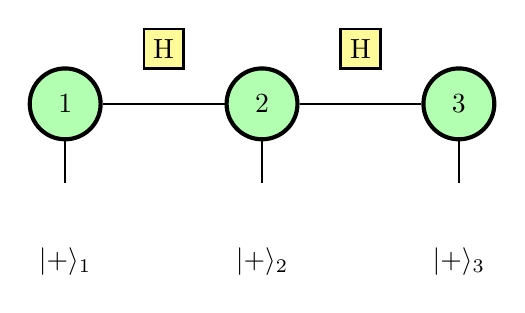
\begin{tikzpicture}[scale=1]
		\node[draw, circle, fill=green!30, minimum size=0.9cm, line width=1.5pt] (g1) at (0,0) {1};
		\node[draw, circle, fill=green!30, minimum size=0.9cm, line width=1.5pt] (g2) at (2.5,0) {2};
		\node[draw, circle, fill=green!30, minimum size=0.9cm, line width=1.5pt] (g3) at (5,0) {3};

		\node[draw, rectangle, fill=yellow!40, minimum size=0.5cm, line width=1pt] (h1) at (1.25,0.7) {H};
		\node[draw, rectangle, fill=yellow!40, minimum size=0.5cm, line width=1pt] (h2) at (3.75,0.7) {H};

		\draw[thick] (g1) -- ++(0,-1) node[below] {};
		\draw[thick] (g2) -- ++(0,-1) node[below] {};
		\draw[thick] (g3) -- ++(0,-1) node[below] {};

		\draw[thick] (g1) -- (g2) -- (g3);


		\node at (0,-2) {$|+\rangle_1$};
		\node at (2.5,-2) {$|+\rangle_2$};
		\node at (5,-2) {$|+\rangle_3$};

	\end{tikzpicture}
	\caption{Graph state representation in ZX calculus. Three qubits prepared in $|+\rangle$ (green spiders) are connected by Hadamard boxes (yellow), forming the graph state. The vertical wires represent the physical qubit outputs.}
	\label{fig:zx-graph-state}
\end{figure}
